%%%%%%%%%%%%%%%%%%%%%%%%%%%%%%%%%%%%%%%%%%%%%%%%%%%%%%%%%%%%
%2345678901234567890123456789012345678901234567890123456789012345678901234567890
%        1         2         3         4         5         6         7         8

\documentclass[letterpaper, 10 pt, conference]{ieeeconf}  % Comment this line out
                                                          % if you need a4paper
%\documentclass[a4paper, 10pt, conference]{ieeeconf}      % Use this line for a4
                                                          % paper

\IEEEoverridecommandlockouts                              % This command is only
                                                          % needed if you want to
                                                          % use the \thanks command
\overrideIEEEmargins
% See the \addtolength command later in the file to balance the column lengths
% on the last page of the document



% The following packages can be found on http:\\www.ctan.org
%\usepackage{graphics} % for pdf, bitmapped graphics files
%\usepackage{epsfig} % for postscript graphics files
%\usepackage{mathptmx} % assumes new font selection scheme installed
%\usepackage{times} % assumes new font selection scheme installed
%\usepackage{amsmath} % assumes amsmath package installed
%\usepackage{amssymb}  % assumes amsmath package installed
\usepackage{graphicx}
\usepackage{verbatim}
\usepackage{multirow}
\usepackage{rotating}
\usepackage{moreverb}                    % for boxedboxedverbatim
\usepackage{array}
\usepackage{fancyvrb}
\usepackage{multicol}
\usepackage{mdwlist}
\usepackage{enumerate}
%\usepackage{tikz-er2}


\newtheorem{defn}{Definition}

\newcommand{\class}[1] {\textit{#1}}
\newcommand{\const}[1] {$\mathit{#1}$}
\newcommand{\objvar}[1] {$\mathsf{#1}$}
\newcommand{\stvar}[1] {\textsf{#1}}
\newcommand{\op}[1] {\textsl{#1}}
\newcommand{\nil} {\textit{nil}\ }

\newcommand\T{\rule{0pt}{2.6ex}}
\newcommand\B{\rule[-1.2ex]{0pt}{0pt}}

%\definecolor{violetred}{cmyk}{0,0.85,0.31,0.18}
%\definecolor{darkblue}{cmyk}{1,1,0,0.45}
%\definecolor{lavenderblush4}{cmyk}{0,0.06,0.04,0.45}
%\definecolor{packergreen}{cmyk}{0.46,0,0.21,0.76}
%\definecolor{fuschia}{cmyk}{0,100,0,0}
%\definecolor{graycmyk}{cmyk}{0,0,0,0.74}
%
%\usetikzlibrary{calc,trees,positioning,arrows,chains,shapes.geometric,%
%    decorations.pathreplacing,decorations.pathmorphing,shapes,%
%    matrix,shapes.symbols,positioning,shadows}
%
%% styles for flowcharts
%
%\tikzstyle{every entity} = [top color=white, bottom color=blue!30,
%                            draw=blue!50!black!100, drop shadow]
%\tikzstyle{empty} = [top color=white, bottom color=white,
%                            draw=white]
%
%\tikzstyle{every weak entity} = [drop shadow={shadow xshift=.7ex,
%                                 shadow yshift=-.7ex}]
%\tikzstyle{every attribute} = [top color=white, bottom color=green!20,
%                               draw=green, node distance=1cm, drop shadow]
%\tikzstyle{ELLIPSE} = [draw, ellipse, top color=white, bottom color=green!20, draw=green, drop shadow]
%\tikzstyle{MainAttribute} = [draw, rectangle,top color=white, bottom color=red!20,
%                               draw=red, node distance=1cm, drop shadow]
%\tikzstyle{DATABASE} = [draw, rectangle, rounded corners,top color=white, bottom color=graycmyk!50, draw=graycmyk, inner sep=10pt, drop shadow={shadow xshift=.7ex, shadow yshift=-.7ex}]
%
%
%\tikzstyle{myarrow}=[->, >=stealth', thick, shorten <=2pt,shorten >=2pt]
%
%
%
%\tikzstyle{output} = [draw, rectangle, rounded corners,top color=white, bottom color=red!30, draw=red, inner sep=10pt, drop shadow={shadow xshift=.7ex, shadow yshift=-.7ex}]
%
%\tikzstyle{abstract}=[rectangle, draw=black, rounded corners, fill=blue!40, drop shadow,
%        text centered, anchor=north, text=white, text width=3cm]
%
%
%\newbox{\LegendOutput}
%\savebox{\LegendOutput}{
%    (\begin{tikzpicture}[]
%    \node[output] (2) {\hspace{5 mm}};
%    \end{tikzpicture}
%    )}


\newenvironment{mylisting}
{\begin{list}{}{\setlength{\leftmargin}{1em}}\item\small}
{\end{list}}

\newenvironment{mytinylisting}
{\begin{list}{}{\setlength{\leftmargin}{1em}}\item\tiny\bfseries}
{\end{list}}


\title{\LARGE \bf
Metrics and Test Methods for Industrial Kit Building
}

%\author{ \parbox{3 in}{\centering Stephen Balakirsky\\
%         Intelligent Systems Division\\
%         National Institute of Standards and Technology\\
%        Gaithersburg, MD 20899, USA\\
%         {\tt\small stephen.balakirsky@nist.gov}}
%         \hspace*{ 0.5 in}
%         \parbox{3 in}{ \centering Zeid Kootbally\\
%          Department of Mechanical Engineering \\
%         University of Maryland\\
%         College Park, MD 20742, USA\\
%         {\tt\small zeid.kootbally@nist.gov}}\\ \\
%	\parbox{2.25 in}{\centering Craig Schlonoff\\
%         Intelligent Systems Division\\
%         National Institute of Standards and Technology\\
%        Gaithersburg, MD 20899, USA\\
%         {\tt\small craig.schlenoff@nist.gov}}
%        \hspace*{0.05in}
%         \parbox{2.25 in}{ \centering Thomas Kramer\\
%          Department of Mechanical Engineering \\
%         Catholic University of America\\
%         Washington, DC 20064, USA\\
%         {\tt\small thomas.kramer@nist.gov}}
%        \hspace*{0.05in}
%         \parbox{2.25 in}{ \centering Satyandra K. Gupta\\
%          Maryland Robotics Center\\
%         University of Maryland\\
%         College Park, MD 20742, USA\\
%         {\tt\small skgupta@umd.edu}}\\
%}

\author{Stephen Balakirsky, Thomas Kramer, and Zeid Kootbally% <-this % stops a space
\thanks{S. Balakirsky is with the Intelligent Systems Division, National Institute of Standards and Technology, Gaithersburg, MD, USA (e-mail:stephen.balakirsky@nist.gov)}% <-this % stops a space
\thanks{Z. Kootbally is with the Department of Mechanical Engineering, University of Maryland, College Park, MD, USA (email: zeid.kootbally@nist.gov)}%
\thanks{T. Kramer is with the Department of Mechanical Engineering, Catholic University of America, Washington, DC, USA (email: thomas.kramer@nist.gov)}%
} 


\begin{document}
\begin {center}
{\huge{Outline}}
\end {center}

\begin{enumerate}
\item SB - Description of kitting
\item Test methods
	\begin{enumerate}
	\item TK -  Inputt format (xml, owl)
	\item TK - Output format (Robot canonical command language)
	\item SB - method itself (build kits) with varying part mix and configuration, missing parts, ...
	\end{enumerate}
\item metrics
	\begin{enumerate}
	\item TK -  Plan
		\begin{enumerate}
		\item number of steps
		\item goal achievement
		\item optimality
		\item maintain constraints
		\item number of errors
		\end {enumerate}
	\item ZK -  Execution
	\end {enumerate}
\item assumptions
	\begin {enumerate}
	\item Work volume totally reachable
	\end {enumerate}
\end{enumerate}


\maketitle
\thispagestyle{empty}
\pagestyle{empty}


%%%%%%%%%%%%%%%%%%%%%%%%%%%%%%%%%%%%%%%%%%%%%%%%%%%%%%%%%%%%
\begin{abstract}

The IEEE RAS Ontologies for Robotics and Automation Working Group is dedicated to 
developing a methodology for knowledge representation and reasoning in robotics 
and automation. As part of this working group, the Industrial Robots sub-group is 
tasked with studying industrial applications of the ontology. One of the first 
areas of interest for this subgroup is the area of kit building or kitting. 
It is anticipated that utilization of the ontology will allow for the development 
of higher performing kitting systems. However, the definition of ``higher performing''
has yet to be defined. This paper addresses this issue by providing the basis 
for performance methods and metrics that are designed to
determine the performance of a kitting system.
\end{abstract}


%%%%%%%%%%%%%%%%%%%%%%%%%%%%%%%%%%%%%%%%%%%%%%%%%%%%%%%%%%%%
\section{INTRODUCTION}
Material feeding systems are an integral part of today's assembly line operations. 
These systems assure that parts are available where and when 
they are needed during the assembly operations by providing either a continuous 
supply of parts at the station, or a set of parts (known
as a 'kit') that contains the required parts for one or more assembly operations. 
In continuous supply, a quantity of each part that
may be necessary for the assembly operation is stored at the assembly station. 
If multiple versions of a product are being assembled, (mixed-model assembly)
a larger variety of parts than are used for an individual assembly may need 
to be stored. With this material feeding scheme, parts
storage and delivery systems must be duplicated at each assembly station.

An alternative approach to continuous supply is known as kitting. In kitting, 
parts are delivered to the assembly station in kits that contain
the exact parts necessary for the completion of one assembly object. 
According to Bozer and McGinnis \cite{Bozer1992} ``A kit is a specific
collection of components and/or subassemblies that together
(i.e., in the same container) support one or more assembly 
operations for a given product or shop order''. In the case of mixed-model
assembly, the contents of a kit may vary from product to product.
The use of kitting allows a single delivery system to feed
multiple assembly stations. The operation of this kitting 
station may be viewed as a specialization of the general bin-picking problem. 

In industrial assembly of manufactured products, kitting is 
often performed prior to final assembly. Manufacturers utilize kitting
due to its ability to provide cost savings \cite{Carlsson_2008} 
including saving manufacturing or assembly space \cite{Medbo2003}, 
reducing assembly workers walking and searching times \cite{Schwind1992}, 
and increasing line flexibility \cite{Bozer1992} and balance \cite{Jiao2000}.

Several different techniques are used to create kits. A kitting 
operation where a kit box is stationary until filled at a single
kitting workstation is referred to as {\it batch kitting}. 
In {\it zone kitting}, the kit moves while being filled and will pass through one or
more zones before it is completed. This paper focuses on batch kitting processes.

In batch kitting, the kit's component parts may be staged in 
containers positioned in the workstation or may arrive on a conveyor.
Component parts may be fixtured, for example placed in compartments 
on trays, or may be in random orientations, for example
placed in a large bin. In addition to the kit's component parts, 
the workstation usually contains a storage area for empty kit boxes as
well as completed kits.

Kitting has not yet been automated in many industries where 
automation may be feasible. Consequently, the cost of building 
kits is higher than it could be. We are addressing this problem 
by proposing performance methods and metrics that will allow for 
the unbiased comparison of various approaches to building kits  
in an agile manufacturing environment. The performance methods 
that we propose must be simple enough to be repeatable at a variety of 
testing locations, but must also capture the complexity inherent 
to variants of kit building. The test methods must address concerns such as
measuring performance against variations in kit contents, kit 
layout, and component supply. For our test methods, we assume that 
a robot performs a series of pick-and-place operations
in order to construct the kit. These operations include:
\begin{enumerate}
\item Pick empty kit and place on work table.
\item Pick multiple component parts and place in kit.
\item Pick completed kit and place in full kit storage area.
\end{enumerate}
Each of these actions may be a compound action that includes 
other actions such as end-of-arm tool changes, path planning,
and obstacle avoidance.

It should be noted that multiple kits may be built simultaneously. 
Finished kits are moved to the assembly floor where components
are picked from the kit for use in the assembly procedure. 
The kits are normally designed to facilitate component picking in the correct
sequence for assembly. Component orientation may be constrained 
by the kit design in order to ease the pick-to-assembly process.
Empty kits are returned to the kit building area for reuse.

\renewcommand{\topfraction}{1.0}
\setcounter{topnumber}{100}

%%%%%%%%%%%%%%%%%%%%%%%%%%%%%%%%%%%%%%%%%%%%%%%%%%%%%%%%%%%%
\section{Test Methods}
\label{sect:TestMethods}
Acording to the American Society for Testing and Materials (ASTM) \cite[p. vii]{ASTM99}, a test method is a
definitive procedure that produces a test result. It is the authors' desire to develop repeatable test methods that will
lead to a better understanding of what it means to have an ``agile" and ``flexible" planning system and metrics that 
will allow for the measurement of a system's agility and flexibility. We have chosen to begin our study
with the domain of kit building since it is a greatly simplified manufacturing/assembly domain. However, 
even in the domain of kit building, there is a large amount of variance that must be accounted for. For
example, will parts be rigid or flexible? Will a vacuum effector, or a parallel jaw mechanism, or a fingered 
gripper be utilized for part picking? Will parts be picked from a tray or a bin? What aspects of the
process will be stressed to demonstrate flexibility and agility?

In keeping with the ideas of reduced complexity and repeatability, we will strive to come up with test methods that stress
the system's agility and not the system's robotic configuration or abilities. As such, we make the following assumptions:
\begin{itemize}
	\item All of the contents of the kit will be rigid objects.
	\item All of the rigid objects are of simple shape (rectilinear) and have a flat surface for a top.
	\item A vacuum effector is utilized for the handling of the parts.
	\item All of the parts will be located in a well-defined parts tray. This will allow for repeatable experiments in terms of part placement.
	\item All of the part's initial and final positions will be within the reach volume of the robot.
	\item There are no obstacles located within the robot's reach volume.
\end{itemize}

\subsection{Test Requirements}
The test methods themselves are designed as a series of tests that have increasing complexity. It is assumed that the tests will be performed
in order, and that a system that is not capable of performing test {\it n} will fail at test {\it n+1} as well. For all of the tests,
the initial condition of the world and the goal kit configurations are provided as XML and/or OWL files conforming with the IEEE RAS Ontologies
for Robotics and Automations Working Group's kitting ontology. The planning system is required to produce an output that
will construct the required kit(s) from the initial condition. All of the commands must be in the form of CRCL, and the system
is allowed to submit new plans that respond to environmental changes.

The parts supply consists of one or more trays of raw materials and
the kit tray is a flat container with separators between locations for individual parts. The part supply trays may be auto-filling (e.g. 
a single location that is continuously fed with a part) or limited quantity trays. Test methods may be configured to require end-of-tool
changes for the picking of various parts.

\subsection{Basic Kit}
The first test method is the construction of a single basic kit. The kit will contain two or more different types of parts. The design of the
kit and parts supply will be known before the test begins. The actual location of the kit tray and parts supplies will not be known before
runtime. The location and orientation (yaw) of the kit and parts supplies will be varied during consecutive runs of the test method.
The planning system is required to submit a single CRCL formated plan that will construct the given kit. There are no execution errors.
Each kit construction will be evaluated by our standard metrics as described in Section \ref{sect:Metrics}. 
This test method will evaluate the following aspects of agility and flexibility:
\begin{itemize}
	\item Ability to correctly build a specific predefined kit.
	\item Agility in terms of part tray and kit placement. Will show that exact fixturing is not necessary for the construction
	of a kit.
	\item If the robot is capable of supporting tool changing, different end-of-arm tooling may be required for grasping
	the various parts.
\end{itemize}

\subsection{New Variety of Basic Kit}
This test provides the system with a never before seen kit variation. The variation will be delivered in the previously
mentioned IEEE RAS OWL/XML format. In addition to the standard kit construction metrics, the time from the receipt
of the new kit configuration to the start of first construction will be recorded. The amount of down-time for the
cell will also be noted. This test will measure the agility of the robot cell in coping with new kit varieties.

\subsection{Basic Kit, Multiple Varieties}
This test builds on the previous test by requiring the construction of two or more kit varieties in a pseudo-random ordering.
The kit configurations will be known before the start of the test. 
This test method will evaluate the following additional aspects of agility and flexibility:
\begin{itemize}
	\item Ability to correctly build several kits with varying part placements without manual intervention.
	This will demonstrate agility in terms of kit layout and contents.
	\item Ability to manipulate items of varying size and weight. This test method will require the workcell
	to move empty kit trays from storage to a construction location and then to move finished kits to
	a bin of finished kits.
	\item If the robot is capable of supporting tool changing, different end-of-arm tooling may be required for 
	kit manipulation. 
\end{itemize}

\subsection{Construction Errors}
This test will evaluate the system's ability to recover from predictable error conditions. These conditions will include
dropped parts and parts with detected defects. It is expected that the planning systems will interrupt the
execution of the kit build in order to provide updated plans to cope with the unexpected events.

%%%%%%%%%%%%%%%%%%%%%%%%%%%%%%%%%%%%%%%%%%%%%%%%%%%%%%%%%%%%


\section{Metrics}
\subsection{Plan Metrics}
\label{sect:PlanMetrics}
\renewcommand{\topfraction}{1.0}
\setcounter{topnumber}{100}

As described in the previous section, a test method is being developed that
will be suitable for comparing the performance of different kitting
planning systems. The method looks at plans that are an ordered sequence
of actions for a robot to perform. The actions are specified in terms of
the canonical robot command language (CRCL).

\subsubsection{Kitting Viewer Introduction}
A software tool named the ``kittingViewer'' is being developed that will
read files describing the initial state, the goal state, and the plan for
getting from the initial state to the goal state. The kittingViewer will
simulate execution of the plan, display a view of the plan being executed,
and produce and display metrics about the plan.  All of the metrics will be
numbers. All but one of the metrics will be objective and require no human
judgement. The final metric will be a subjective combination of the other
metrics in which the other metrics will be weighted and combined as desired
by the user.

The kittingViewer is partially built. It is able to read in the three
input files and simulate execution of the plan file. Plan metrics are
being calculated, and robot motion is being animated at speeds specified
in the plan.

A sample plan file is shown in Figure~\ref{fig:KittingPlan}. The file is
designed for exercising the kittingViewer and is not intended to make sense
as a plan. It includes a few intentional errors.

Figure~\ref{fig:KittingViewer} shows the kittingViewer display at its
current state of development. The display uses three windows, labelled
Metrics \& Settings, Kitting Viewer, and Kitting Command. The windows may
be moved and resized independently, like other windows in a typical
windowing system. The image in the Kitting Viewer window resizes when the
window is resized, but the text in the other two windows does not
change size when the windows change size, so there is little point in
resizing them.

The Kitting Viewer window shows a view of the kitting workstation. The
floor of the workstation is covered with a grid. The spacing of the grid is
the last entry in the Metrics and Settings window. The robot in the
workstation is represented by a gantry robot spanning the entire width of
the workstation.  The gantry robot moves when any of the CRCL motion
commands is executed.  The speed at which the picture of the robot is
animated matches the actual commanded speed of the robot.  When development
of the kittingViewer is complete, objects in the workstation will also be
shown (in color) and will move if the robot moves them.

The Kitting Command window shows the currently executing command or the
most recently executed command, if no command is currently executing.

\begin{figure*}[ht]
\begin{center}
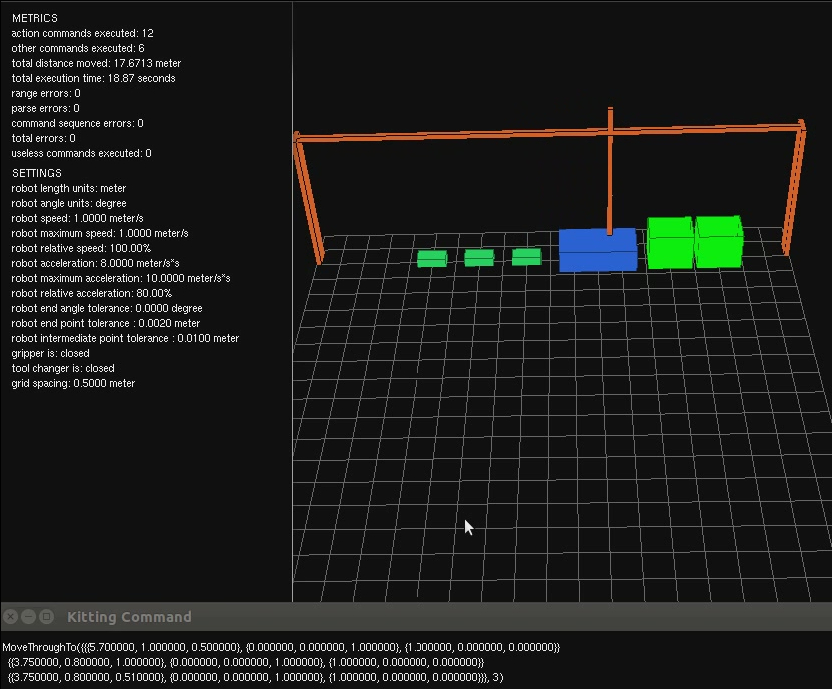
\includegraphics[width=16cm]{images/kittingViewer.jpg}
\caption{Kitting Viewer Display}
\label{fig:KittingViewer}
\end{center}
\end{figure*}

\subsubsection{Kitting Viewer Metrics}
The Metrics \& Settings window shows 9 metrics at the top and 14 settings
below that. All but three of the settings correspond to items that may be
set using CRCL commands. The extra three are the grid spacing and the robot
maximum speed and maximum acceleration (which may not be reset). As
commands are executed, metrics and settings are updated in the window.
When the kittingViewer is completed, there will be more metrics.
Currently, the metrics are:\\

\begin{itemize}

\item \sf action commands executed \rm -- the number of action commands that
  have been executed so far. An action command is any command that takes
  time to execute, namely: Dwell, MoveStraightTo, MoveThroughTo, MoveTo,
  OpenGripper, CloseGripper, OpenToolChanger, and CloseToolChanger.\\

\item \sf other commands executed \rm -- the number of commands that are
  not action commands and have been executed so far -- mostly setting
  commands. Executing these commands is assumed to take a negligible amount
  of time.\\

\item \sf total distance moved \rm -- the total distance covered so
  far. This is calculated as the total of the distances between points in
  the move commands, taken in order (and starting at the place where the
  controlled point is located initially). The value is updated as each point
  is reached, not continuously.\\

\item \sf total execution time \rm -- the total time taken so far by
  executing action commands. This does not include any time that may elapse
  between when one command finishes execution and when the user tells the
  kittingViewer to execute another command. The total execution time is
  meant to be very close to the actual amount of time that would be taken
  by a real robot.\\

\item \sf range errors \rm -- the number of times a command tries to set a
  value that is out of the allowed range of the value. If a range error
  occurs, an error message is printed in the terminal window from which the
  kittingViewer was started. The \sf SetRelativeAcceleration(-110) \rm
  command in Figure~\ref{fig:KittingPlan} causes two range errors, one
  because it is negative, and one because its absolute value is greater
  than 100.\\

\item \sf parse errors \rm -- the number of lines in the CRCL command file
  that cause an error in the command file parser. When the parser
  encounters a line that it cannot parse, it adds an UnreadableMsg to the
  list of commands it has parsed. The UnreadableMsg includes the text of
  the line on which the parse error occurred. When the UnreadableMsg is
  executed, the value of parse errors is increased by one and the
  UnreadableMsg is displayed in the Kitting Command window so the user can
  see the line that caused the problem. The \sf MoveStraightTo(87) \rm
  command in Figure~\ref{fig:KittingPlan} causes a parse error.\\

\item \sf command sequence errors \rm -- the number of commands that are
  out of sequence. An InitCanon command is out of sequence if it is not the
  first command in the file. An EndCanon command is out of sequence if it
  is not the last command in the file. Other commands are out of sequence
  if they occur before InitCanon or after EndCanon.\\

\item \sf total errors \rm -- the sum of the range errors, parse errors,
  and command sequence errors.\\

\item \sf useless command executed \rm -- the number of commands that do
  not change the state of the workstation. Such commands have no effect, so
  they are useless. The \sf CloseGripper() \rm and \sf CloseToolChanger()
  \rm commands in Figure~\ref{fig:KittingPlan} are useless because the
  gripper and tool changer are closed in the initial conditions.\\

\end{itemize}

\subsubsection{Controlling Kitting Viewer}
Controlling the kittingViewer is accomplished by using the mouse and single
keys on the keyboard. When the kittingViewer starts up, a set of one-line
instructions is printed in the terminal window from which the
kittingViewer was started. Those instructions have the same meaning as
the longer explanations given below.\\

\begin{itemize}

\item R key -- The R key toggles the behavior of the left mouse button
  between translating and rotating the picture. This functionality is
  included because some mice do not have a middle button. Press R once and
  the left mouse button controls rotation. Press R again and the the left
  mouse button controls translation (the original setting).\\

\item Left mouse button -- By default, the left mouse button is used to
  translate the picture. Position the cursor anywhere in the Kitting Viewer
  window, hold down the left mouse button and move the cursor by moving the
  mouse. The picture will move as though it is glued to the cursor. If the
  R key has switched the left mouse button to rotation, it behaves like the
  middle mouse button, as described in the next paragraph.\\

\item Middle mouse button -- The middle mouse button is used to rotate the
  picture. This is a little trickier than the other two mouse buttons. To
  rotate the picture, position the cursor inside the window near an edge of
  the window, hold down the middle mouse button, and move the cursor in a
  straight line towards the opposite edge. The picture rotates around an axis
  that is perpendicular to the line of mouse motion. Experiment. In order
  to allow for fine positioning, the amount of rotation that occurs for a
  given amount of mouse motion decreases as the picture is zoomed
  in. Hence, if you want to turn the picture completely over, it is best to
  zoom out, rotate, and zoom back in again.\\

\item Right mouse button -- The right mouse button is used to zoom in or
  out. To zoom out, position the cursor near the bottom of the picture,
  hold down the right mouse button and push the mouse away from you (moving
  the cursor up); that appears to push the picture away from you. To zoom
  in, position the cursor near the top of the picture, hold down the right
  mouse button and pull the mouse toward you (moving the cursor down); that
  appears to pull the picture toward you. Moving the mouse side to side
  while holding down the right mouse button does nothing. There are limits
  to how far in or out you can zoom. At the highest magnification, it is
  easy to see a separation of half a millimeter. This is zooming, not
  moving the point of view, so the eye never goes through the picture.\\

\item H key -- If the h key is pressed, the view in the Kitting Viewer
  window returns to its original position.\\

\item G key -- If the g key is pressed when the plan is not completely
  executed and no action command is executing, the next command in the plan
  is executed and the Metrics \& Settings window is updated. If the g key
  is pressed when the plan is completely executed or when an action command
  is in progress, nothing happens.\\

\item T key -- If the t key is pressed, a combined image of all the windows
  will be saved in a file. The name of the file will be anaglyph\_N.ppm,
  where N starts at 0000 and increases by 1 each time the t key is
  pressed. The ppm (portable pixmap) format is a common graphics format
  that many graphics utilities can handle.\\

\item Z or Q key -- If the z or q key is pressed, the kittingViewer program
  exits, and the windows disappear.\\

\end{itemize}

\subsubsection{Kitting Viewer Development Plans}

As mentioned earlier, the kittingViewer is far from complete. It is
planned to add the following capabilities.

\begin{itemize}

\item Add drawing the kitting workstation in its current state. The initial
  state of the workstation is already available in data as soon as the XML
  data file that describes it is read in. 

\item Add updating the positions of objects as the robot executes commands.
  It will be necessary to compare the position of the robot with the
  positions of objects when OpenGripper and CloseGripper commands are
  executed in order to determine if the robot is grasping them.

\item Add metrics related to the positions of objects. This might include
  (1) the number of objects that should have been moved, (2) the number of
  objects that were moved (3) the number of objects that were moved to the
  correct place, (4) the number of objects that were moved to the wrong
  place.

\item Add metrics related to constraint violations. This might include (1)
  the number of instances of picking up an object that weighs more than the
  robot's load capacity, (2) the number of instances of the robot moving
  outside of its work volume, (3) the number of instances of using a
  gripper to move an object when the gripper is not qualified to move the
  object. It will also be necessary to decide what the simulation should do
  in these cases and implement that.

\item Add a total score metric, and implement finding the total score using
  a configuration file in which the user assigns weights to the other
  metrics.

\end{itemize}

\subsection{Execution Metrics}
\label{sect:ExecutionMetrics}
The kitting system presented in this document relies on a \textit{direct} model of execution where the executor directly performs the activities specified in the plan. Figure~\ref{fig:executor} depicts the executor process for the kitting domain where ellipses represent files, regular rectangles are used to define processes, and rounded rectangles illustrate tools. The red dashed box contains the processes part of the executor. The components in Figure~\ref{fig:executor} are described below:
\begin{itemize}
\item[$1.$] PDDL domain and problem files are used by a planner to generate a plan file. The plan file contains a sequence of actions that can be executed from the initial state and that leads to a goal state. The actions present in the plan file are originally defined in the PDDL domain file. The initial and goal states are defined in the PDDL problem file.
\item[$2.$] The interpreter takes the plan file as input and builds the corresponding CRCL file. The knowledge representation is required to locate objects in the environment. Table~\ref{tab:takepart} shows an example of CRCL commands generated for the PDDL action \stvar{take-part(part\_b\_1)}. Please note that the PDDL action \stvar{take-part} developed for the current kitting domain has more than one parameter. All the parameters are not relevant for the example depicted in Table~\ref{tab:takepart} and the number of parameters has been subsequently reduced for simplicity.

\begin{table}[h!]
\centering

    \begin{tabular}{l}
    \stvar{take-part(part\_b\_1)}\\
    \hline
    \hline
  \texttt{\scriptsize{Message (``take part part\_b\_1")}}\\
  \texttt{\scriptsize{MoveTo(\{\{-0.03, 1.62, -0.25\}, \{0, 0, 1\}, \{1, 0, 0\}\})}}\\
  \texttt{\scriptsize{Dwell (0.05)}}\\
  \texttt{\scriptsize{MoveTo(\{\{-0.03, 1.62, 0.1325\}, \{0, 0, 1\}, \{1, 0, 0\}\})}} \\
  \texttt{\scriptsize{CloseGripper ()}} \\
  \texttt{\scriptsize{MoveTo(\{\{-0.03, 1.62, -0.25\}, \{0, 0, 1\}, \{1, 0, 0\}\})}}\\
  \texttt{\scriptsize{Dwell (0.05)}}\\
  \hline
  \end{tabular}
\caption{An example of CRCL commands for a PDDL action.}
  \label{tab:takepart}
\end{table}
\item[$3.$] The CRCL file is used by the controller in order to create ROS commands.
\item[$4.$] The ROS commands are used by the ROS software controller for a robotic arm to initiate actual execution of actions.

\end{itemize}

%The \textit{indirect} model tracks the execution of the plan while human agents perform the plan activities. Both models of execution require tools to monitor failures that are likely to emerge during a plan execution.



\begin{figure}[h!]
\centering
\scalebox{.7}{
\begin{tikzpicture}[node distance=1.5cm, every edge/.style={link}]

  %%-- Domain file
  \node[attribute] (domain) {PDDL Domain};
  %%-- Empty node to center the planner node that comes right below it
  \node[empty] (empty) [right=0.5cm of domain]{};
  %%-- Problem file
  \node[attribute] (problem) [right=0.5cm of empty] {PDDL Problem};
  %%-- Planner
  \node[entity] (planner) [below=1cm of empty] {$1.$ Planner};
  %%-- Plan
  \node[attribute] (plan) [below=0.5cm of planner] {Plan};
  %%-- Knowledge Representation
  \node[output] (database) [left=1cm of plan] {Knowledge Representation};
  %%-- Interpreter
  \node[entity] (interpreter) [below=1cm of plan] {$2.$ Interpreter};
  %%-- CRCL
  \node[attribute] (crcl) [below=0.5cm of interpreter] {CRCL};
  %%-- Controller
  \node[entity] (controller) [below=0.5cm of crcl] {$3.$ Controller};
  %%-- ROS commands
  \node[entity] (ros) [below=1cm of controller] {$4.$ ROS};
  %%-- Robotic Arm
%  \node[output] (arm) [below=1cm of ros] {Robotic Arm};

  \draw[myarrow] (domain.south) -- ++ (0,-1)  |-  (planner.west);
  \draw[myarrow] (problem.south) -- ++ (0,-1)  |-  (planner.east);
  \draw[myarrow] (planner.south) -- (plan.north);
  \draw[myarrow] (plan.south) -- (interpreter.north);
  \draw[myarrow] (interpreter.south) -- (crcl.north);
  \draw[myarrow] (crcl.south) -- (controller.north);
  \draw[myarrow] (controller.south) -- (ros.north);
  %\draw[myarrow] (ros.south) -- (arm.north);
  %\draw[thick,decorate,decoration={brace,amplitude=10pt,mirror,raise=4pt},yshift=0pt]
  %     (4.5,-10) -- (4.5,-4.2) node[midway, right=15pt]{Executor};
  \draw[myarrow] (database.south) -- ++ (0,-1)  |-  (interpreter.west);

  %\draw[red,thick,dotted] ($(interpreter.north west)+(-0.5,0.6)$)  rectangle ($(controller.south east)+(0.5,-0.6)$) node [rotate=90, right=of interpreter] {Executor};
  \draw[red,thick,dotted] ($(interpreter.north west)+(-0.5,0.6)$)  rectangle ($(controller.south east)+(0.5,-0.6)$);

\end{tikzpicture}
}
\caption{The executor process.}
\label{fig:executor}
\end{figure}



During execution, kitting fails to reach its full potential for savings when the supply chain fails and parts and components are not available for kit construction, or when a kit is not properly filled. Part availability failures can be triggered by inaccurate information on the location of the part or part shortage due to delays in internal logistics. Kit construction errors may be due to problems such as improper equipment setup, improper equipment maintenance, part damage, wrong type of part, or part dropped by the robot.


Models for detecting and recovering from plan execution failures mostly deal with \textit{precondition failures}, \textit{action failures}, and \textit{unattributable failures}~\cite{Myers1998}. Precondition failures appear when all the preconditions for a PDDL action are not met during the execution of this action. Action failures are encountered when the execution of an action does not attain its intended effects. Unattributable failures occur when unexpected events caused by external agents change a random part of the environment, thus causing the current plan to become obsolete.

Some metrics revolving around the three aforementioned failure concepts are listed below:
\begin{itemize}
\item \sf Manipulation robustness \rm -- Qualitative functionality metrics that describe how well a robot can handle complex objects in complex environments without failing or requiring additional operator interventions. Failures can occur during object detection (lightning variation, shadows), object approach (partially buried), and object manipulation (fragile) operations.\\
\item \sf Transporting components \rm -- Qualitative metrics that describe how well a robotic arm can grasp objects and move these objects from an initial position to a goal position without dropping them.\\
\item \sf Plan generation \rm -- As mentioned previously, failures are susceptible to happen in kitting during the execution of CRCL commands, causing the current plan to become obsolete. In some cases, the current state of the environment is brought back to the state prior to the failure and the robot starts from a ``stable" state. In other cases a completely new plan is generated by the planning system where the robot starts all over. Previous experience suggests that the latter solution is preferable considering it will take less time to generate a new plan than going back to a previous state from the original plan.

    However, the state of the environment after a failure may be closer to the goal configuration and a complete replanning may take longer. In this case, the most time effective action sequence that leads to the goal state is used by the system.\\
\item \sf Contact errors \rm -- Quantitative metrics that keep track of the number of collisions between the robotic arm and objects in the environment. The performance of the robotic arm during kit building is affected by the position of joints and end-effector in the environment. The position of the end-effector can reduce the time to complete tasks but can also increase the number of collisions due to joint contact with other objects in a confined space.\\
%\item \sf Action effects \rm -- Table~\ref{tab:takepart} represents the PDDL action . \\
\item \sf Failures during kit building\rm -- Quantitative metrics the report the total number of failures encountered during kit building. When a failure arises during the building of a kit, the system may generate a new plan to recover from the failure. If a failure occurs during the execution of the new plan, different or not from the previous one, the number of failures for building the current kit is incremented and this number is now 2. The number of failures for building a kit is not related to the plan itself but with the construction of the finished kit. \\
\item \sf Failure modes recovery \rm -- Quantitative metrics that represent the number of failure modes the system recovers from through the use of contingency plans. When a failure is detected in the execution process, failure monitors encode appropriate responses (contingency plans) to failure modes for this particular failure.\\

\end{itemize}



%%%%%%%%%%%%%%%%%%%%%%%%%%%%%%%%%%%%%%%%%%%%%%%%%%%%%%%%%%%%


\section{Assumptions}
\label{sect:Assumptions}
Blah, Blah, Blah

\addtolength{\textheight}{-15cm}   
                                  % This command serves to balance the column lengths
                                  % on the last page of the document manually. It shortens
                                  % the textheight of the last page by a suitable amount.
                                  % This command does not take effect until the next page
                                  % so it should come on the page before the last. Make
                                  % sure that you do not shorten the textheight too much.

%%%%%%%%%%%%%%%%%%%%%%%%%%%%%%%%%%%%%%%%%%%%%%%%%%%%%%%%%%%%%%%%%%%%%%%%%%%%%%%%

%%%%%%%%%%%%%%%%%%%%%%%%%%%%%%%%%%%%%%%%%%%%%%%%%%%%%%%%%%%%
\section{CONCLUSIONS AND FUTURE WORK}
\label{sect:Conclusions}


\bibliographystyle{plain}
\bibliography{kitting}
\end{document}
